\documentclass[tikz,border=1pt]{standalone}

\usepackage{pgfplots}
\pgfplotsset{compat=1.18}

\begin{document}

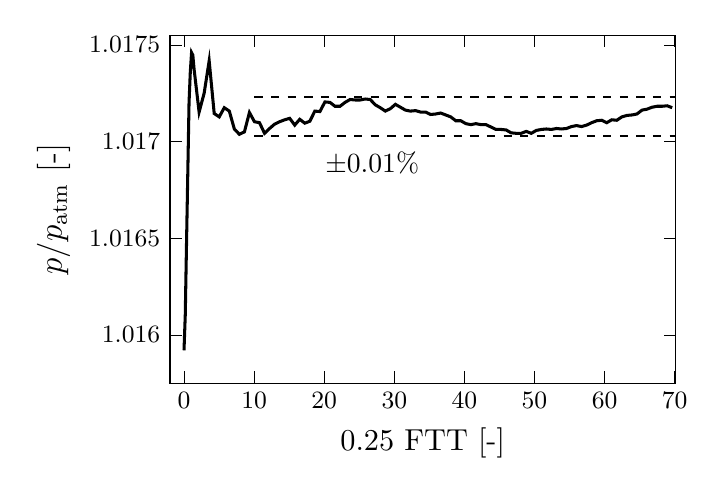
\begin{tikzpicture}
\begin{axis}[
    width=8.0cm,
    height=6.0cm,
    xmin=-2, xmax=70.1,
    ymin=1.01575, ymax=1.01755,
    xlabel={0.25 FTT [-]},
    ylabel={$p/p_\mathrm{atm}$ [-]},
    xlabel style={font=\fontsize{11pt}{12pt}\selectfont},
    ylabel style={font=\fontsize{12pt}{12pt}\selectfont},
    % label style={font=\large},
    tick align=inside,
    tick style={black},
    minor tick num=0,
    % xtick={0,0.2,0.4,0.6,0.8,1.0},
    % ytick={1.0160,1.0165,1.0170,1.0175},
    xticklabel style={font=\fontsize{9.5pt}{12pt}\selectfont},
    yticklabel style={
        /pgf/number format/fixed,
        /pgf/number format/precision=4,
        font=\fontsize{9.5pt}{10pt}\selectfont
    },
    scaled y ticks=false,
    % grid=both,
    % major grid style={gray!45,dashed,line width=0.4pt},
    % minor grid style={gray!25,dashed,line width=0.25pt},
    axis line style={black},
]

\def\xscale{70}

\addplot[
    black,
    line width=1.1pt,
    mark=none
]
table[row sep=\\, x expr=\thisrow{x}*\xscale, y=y] {
x y \\
0.00000 1.0159200 \\
0.00256 1.0161025 \\
0.00513 1.0164750 \\
0.00769 1.0168350 \\
0.01026 1.0172025 \\
0.01282 1.0173600 \\
0.01538 1.0174600 \\
0.01795 1.0174475 \\
0.02051 1.0173750 \\
0.03077 1.0171525 \\
0.04103 1.0172500 \\
0.05128 1.0174175 \\
0.06154 1.0171450 \\
0.07179 1.0171275 \\
0.08205 1.0171750 \\
0.09231 1.0171575 \\
0.10256 1.0170650 \\
0.11282 1.0170375 \\
0.12308 1.0170500 \\
0.13333 1.0171500 \\
0.14359 1.0171025 \\
0.15385 1.0170975 \\
0.16410 1.0170425 \\
0.17436 1.0170675 \\
0.18462 1.0170900 \\
0.19487 1.0171025 \\
0.20513 1.0171125 \\
0.21538 1.0171200 \\
0.22564 1.0170850 \\
0.23590 1.0171150 \\
0.24615 1.0170950 \\
0.25641 1.0171050 \\
0.26667 1.0171575 \\
0.27692 1.0171550 \\
0.28718 1.0172050 \\
0.29744 1.0172025 \\
0.30769 1.0171825 \\
0.31795 1.0171825 \\
0.32821 1.0172025 \\
0.33846 1.0172175 \\
0.34872 1.0172150 \\
0.35897 1.0172150 \\
0.36923 1.0172200 \\
0.37949 1.0172175 \\
0.38974 1.0171900 \\
0.40000 1.0171750 \\
0.41026 1.0171575 \\
0.42051 1.0171700 \\
0.43077 1.0171925 \\
0.44103 1.0171775 \\
0.45128 1.0171625 \\
0.46154 1.0171575 \\
0.47179 1.0171600 \\
0.48205 1.0171525 \\
0.49231 1.0171525 \\
0.50256 1.0171400 \\
0.51282 1.0171425 \\
0.52308 1.0171475 \\
0.53333 1.0171375 \\
0.54359 1.0171275 \\
0.55385 1.0171075 \\
0.56410 1.0171075 \\
0.57436 1.0170925 \\
0.58462 1.0170875 \\
0.59487 1.0170925 \\
0.60513 1.0170875 \\
0.61538 1.0170875 \\
0.62564 1.0170750 \\
0.63590 1.0170625 \\
0.64615 1.0170625 \\
0.65641 1.0170600 \\
0.66667 1.0170450 \\
0.67692 1.0170425 \\
0.68718 1.0170425 \\
0.69744 1.0170525 \\
0.70769 1.0170425 \\
0.71795 1.0170575 \\
0.72821 1.0170625 \\
0.73846 1.0170650 \\
0.74872 1.0170625 \\
0.75897 1.0170675 \\
0.76923 1.0170650 \\
0.77949 1.0170675 \\
0.78974 1.0170775 \\
0.80000 1.0170825 \\
0.81026 1.0170775 \\
0.82051 1.0170850 \\
0.83077 1.0170975 \\
0.84103 1.0171075 \\
0.85128 1.0171100 \\
0.86154 1.0170975 \\
0.87179 1.0171125 \\
0.88205 1.0171100 \\
0.89231 1.0171275 \\
0.90256 1.0171350 \\
0.91282 1.0171375 \\
0.92308 1.0171425 \\
0.93333 1.0171625 \\
0.94359 1.0171675 \\
0.95385 1.0171775 \\
0.96410 1.0171825 \\
0.97436 1.0171825 \\
0.98462 1.0171850 \\
0.99487 1.0171750 \\
};

\def\pref{1.01713}
\def\tol{0.0001} % 0.01%

% +0.01% horizontal dashed line
\addplot[
    black,
    dashed,
    line width=0.8pt,
    domain=10.05:70.05,
    samples=2
] {\pref*(1+\tol)};

% -0.01% horizontal dashed line
\addplot[
    black,
    dashed,
    line width=0.8pt,
    domain=10.05:70.05,
    samples=2
] {\pref*(1-\tol)};

% label below the lower dashed line
\node[
    anchor=north west,
    font=\fontsize{10pt}{10pt}\selectfont,
    yshift=-2pt,
    xshift=45pt
] at (axis cs:1.0,{\pref*(1-\tol)}) {$\pm 0.01\%$};

\end{axis}
\end{tikzpicture}

\end{document}